\documentclass[12pt,letterpaper,oneside]{article}

% The file intend to keep track of good practices in Latex writing.

%==============================
% DOCUMENT
%==============================

% Fix some error reporting
\vfuzz2pt % Don't report over-full v-boxes if over-edge is small
\hfuzz2pt % Don't report over-full h-boxes if over-edge is small

% All the same, there are commands, classes and packages which are outdated and superseded. 
% nag provides routines to warn the user about the use of those.
\usepackage[l2tabu,orthodox]{nag}

%==============================
% BIBLIOGRAPHY
%==============================

% \addbibresource{references.bib} % in your preamble
% \citet{key}, \citep{key} % in the document
% \printbibliography % to generate the reference section
\usepackage[
backend=bibtex8, 
style=ieee, 
sorting=none, 
natbib=true, 
doi=false, 
isbn=false, 
url=false, 
eprint=false, 
maxcitenames=1, 
mincitenames=1
]{biblatex}

%==============================
% TEXT
%==============================

% \autoref{key} % instead of Figure~\ref{key}, Table~\ref{key}, Equation~\ref{key}, or Section~\ref{key}
\usepackage[pdftex,colorlinks]{hyperref}
% fix names for autoref
\def\sectionautorefname{Section}
\def\subsectionautorefname{Section}
\def\subsubsectionautorefname{Section}
\newcommand*{\Appendixautorefname}{Appendix}

% \acrodef{ICP}{Iterative Closest Point} % in the preamble
% \ac{ICP} % in the document
\usepackage[printonlyused]{acronym}

% International unit system 
% e.g., \SI{1000}{\m\squared}, \num{20000}
\usepackage{siunitx}
\sisetup{group-separator = \text{\,}} % small space for thousand separator

% avoid single line on a page or single line under a figure
% no command to use
\usepackage[all]{nowidow}

% Colored text
\usepackage[dvipsnames]{xcolor}

% Fill the template with text
\usepackage{lipsum}

% Better command to make sure that people don't confuse lipsum text with real text
\newcommand{\lightlipsum}[1][0]{\textcolor{gray!50}{\lipsum[#1]}}

%==============================
% FIGURE
%==============================

% Preferred figure format:
% - pdf or eps for graphs and schemas
% - jpg for photo
% Don't use png as each compilation decompress the image, thus making compilation time
% untolerable when there are more than 5 images...

% \includegraphics[width=\textwidth]{filename}
\usepackage[pdftex]{graphicx}

% convert eps to pdf, you need to skip the file extension to work properly
% \includegraphics{filename} % instead of \includegraphics{filename.eps}
\usepackage{epstopdf}

% for Inkscape figures, import tex files in other folder and keep paths coherent
% e.g., \import{images}{timeline.pdf_tex}
\usepackage{import}

% include path for logos
\graphicspath{{./figures/}}

%==============================
% TABLE
%==============================

% Cleaner spacing for tables
% \toprule, \midrule, \bottomrule % instead of \hline
\usepackage{booktabs}

% Tables that can fit page length
% e.g.,three columns with the second one being twice as large as the others
% \begin{tabu}{X X[2] X}
\usepackage{tabu}

%==============================
% MATH
%==============================

% Better symboles
\usepackage{amssymb,amsfonts,amsmath,amscd}

% \bm % in equations for proper bold font
\usepackage{bm} 

% Some handy commands
\newcommand{\norm}[1]{\left\Vert#1\right\Vert}
\newcommand{\abs}[1]{\left\vert#1\right\vert}
\newcommand{\set}[1]{\left\{#1\right\}}
\newcommand{\Real}{\mathbb R}
\newcommand{\bbm}{\begin{bmatrix}}
\newcommand{\ebm}{\end{bmatrix}}




%==============================================================
% FILL THIS SECTION

\newcommand{\reportTitle}{Getting started with HD2 - Marmotte}
\newcommand{\reportAuthors}{Nicolas Antonucci}
\newcommand{\reportDate}{\today} % or manually: November 23, 2017

\newcommand{\reportVersions}{
0.1 & \today & Initial writing %\\
%1.0 & November 23, 2017 & Final writing
}
% Change to your specific bibliography file
\addbibresource{./latexGoodPractices/exampleReferences.bib}
%\addbibresource{./references.bib}
%==============================================================




% ---------------------------------------------------------------
% Load style
%----------------------------------------
% Page style

% Set the page size
\addtolength{\hoffset}{-0.75in} \addtolength{\voffset}{-0.75in}
\setlength{\textwidth}{7in} \setlength{\textheight}{8.25in}
\setlength{\headheight}{0.6in}
\setlength{\headsep}{0.2in}

\setlength{\footskip}{40pt}
\setlength{\fboxsep}{12pt}

% Set the paragraph skip
\setlength{\parskip}{3pt}

% Access to a counter for the number of pages
\usepackage{lastpage}

% To allow text justify on the right
\usepackage{ragged2e}

%----------------------------------------
% Title style

\newcommand{\makeCustomTitle}
{
\begin{center}
\LARGE{\textbf{\reportTitle{}}}
\\
\vspace{5pt}
\normalsize{\reportAuthors{}}
\\
\reportDate{}
\end{center}
\begin{flushright}
\footnotesize{
\begin{tabu}{ccX}
\toprule
\emph{Version} & \emph{Date} & \emph{Comments} \\
\midrule
\reportVersions{} \\
\bottomrule
\end{tabu}
}
\end{flushright}
}

%----------------------------------------
% Section style
\usepackage{sectsty}

% Set the section labeling font
\allsectionsfont{\textsf\bfseries}

%----------------------------------------
% Caption style
\usepackage[font=small, labelfont=bf, skip=5pt]{caption}

%----------------------------------------
% header style
\usepackage{fancyhdr}



% Define the title page style
\fancypagestyle{titlePage}{%
\fancyhf{}%

\fancyhead[L]{
\includegraphics[height=0.45in]{UL_N}}
\fancyhead[C]{\raisebox{0.2in}{\textsc{Technical Report}}}
\fancyhead[R]{
\includegraphics[height=0.45in]{norlab_logo_acronym_dark}}
\fancyfoot[C]{\thepage/\pageref*{LastPage}}

\renewcommand{\headrulewidth}{0.1pt}
\renewcommand{\footrulewidth}{0.2pt}
}

% Define the page style for the other pages
\fancypagestyle{plain}{%
\fancyhf{}
\fancyhead[L]{\reportTitle{}}
\fancyfoot[C]{\thepage/\pageref*{LastPage}}
\renewcommand{\headrulewidth}{0.1pt}
\renewcommand{\footrulewidth}{0.1pt}
}

% Set the page style for all the document except the first page
\pagestyle{plain}

%----------------------------------------
% footnote style
\usepackage{fnpos}
% Fix the footnotes location
\makeFNbottom \makeFNbelow

% ---------------------------------------------------------------
% Author

\author{\reportAuthors{} \\
       Laval University\\
       1065, av. de la Médecine \\
       Quebec, Qc \\
       Canada G1V 0A6 \\
}

% ---------------------------------------------------------------
% PDF setup
\hypersetup{
    pdftitle={\reportTitle},
    pdfauthor={\@author},
    pdfkeywords={research, project, robotics, norlab, Northern Robotics Lab, Master's},
    pdfsubject={},
    pdfstartview={},
    urlcolor=cyan,
    linkcolor=red,
}
% ---------------------------------------------------------------


% Add your other packages here
% make sure to check prembule.tex first!



%================================================================
\begin{document}
\makeCustomTitle
\thispagestyle{titlePage}

% ---------------------------------------------------------------
\begin{abstract}
This is a short technical report to help me get familiar with the project and have all the important information and specifications relative to my task in one place.
\end{abstract}

% ---------------------------------------------------------------
\section{HD2 Treaded Tank Robot Platform}

\begin{figure}[h]
    \centering
    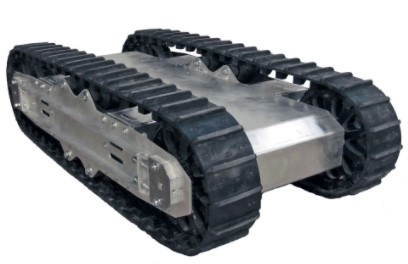
\includegraphics[width=0.4\textwidth]{./figures/platform.jpg}
    \caption{Robot platform}
    \label{fig:my_label}
\end{figure}

\begin{itemize}
    \item From superdroidrobots.com
    \item Can climb obstacles, ascend stairs and drive over most terrain
    \item Controled through Roboclaw motor controller
    \item We use 4 IG52-04 24VDC 285 RPM Gear Motor, 2 of them with encoders. Encoders are not needed for the other 2 as they are connected in line with the same track
\end{itemize}

\begin{figure}[h]
    \centering
    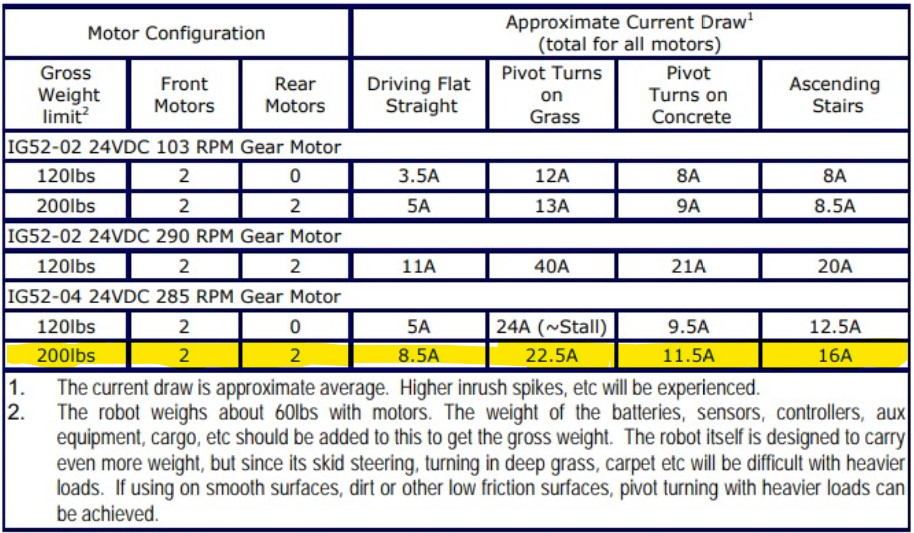
\includegraphics[width=0.8\textwidth]{figures/motorSpecs.jpg}
    \caption{Motor config}
    \label{fig:my_label}
\end{figure}

% ---------------------------------------------------------------
\newpage
\section{D.C. Geared motors}%

\begin{itemize}
    \item Name: IG52-04 24VDC 285 RPM Gear Motor
    \item Variable speed and reversible
    \item Dual channel quadrature encoder
    \item \textbf{Each channel requires a 1k pull up resistor to Vcc}
\end{itemize}

\begin{tabular}{ c c }
    Motor & Pull up resistor attached \\
    %\hline
     \raisebox{-\totalheight}{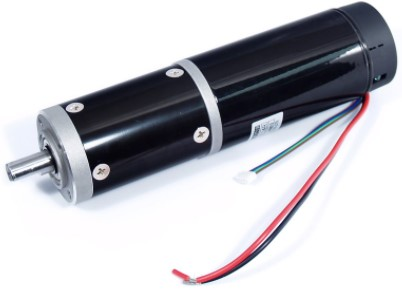
\includegraphics[width=0.45\textwidth]{figures/motor.jpg}} & \raisebox{-\totalheight}{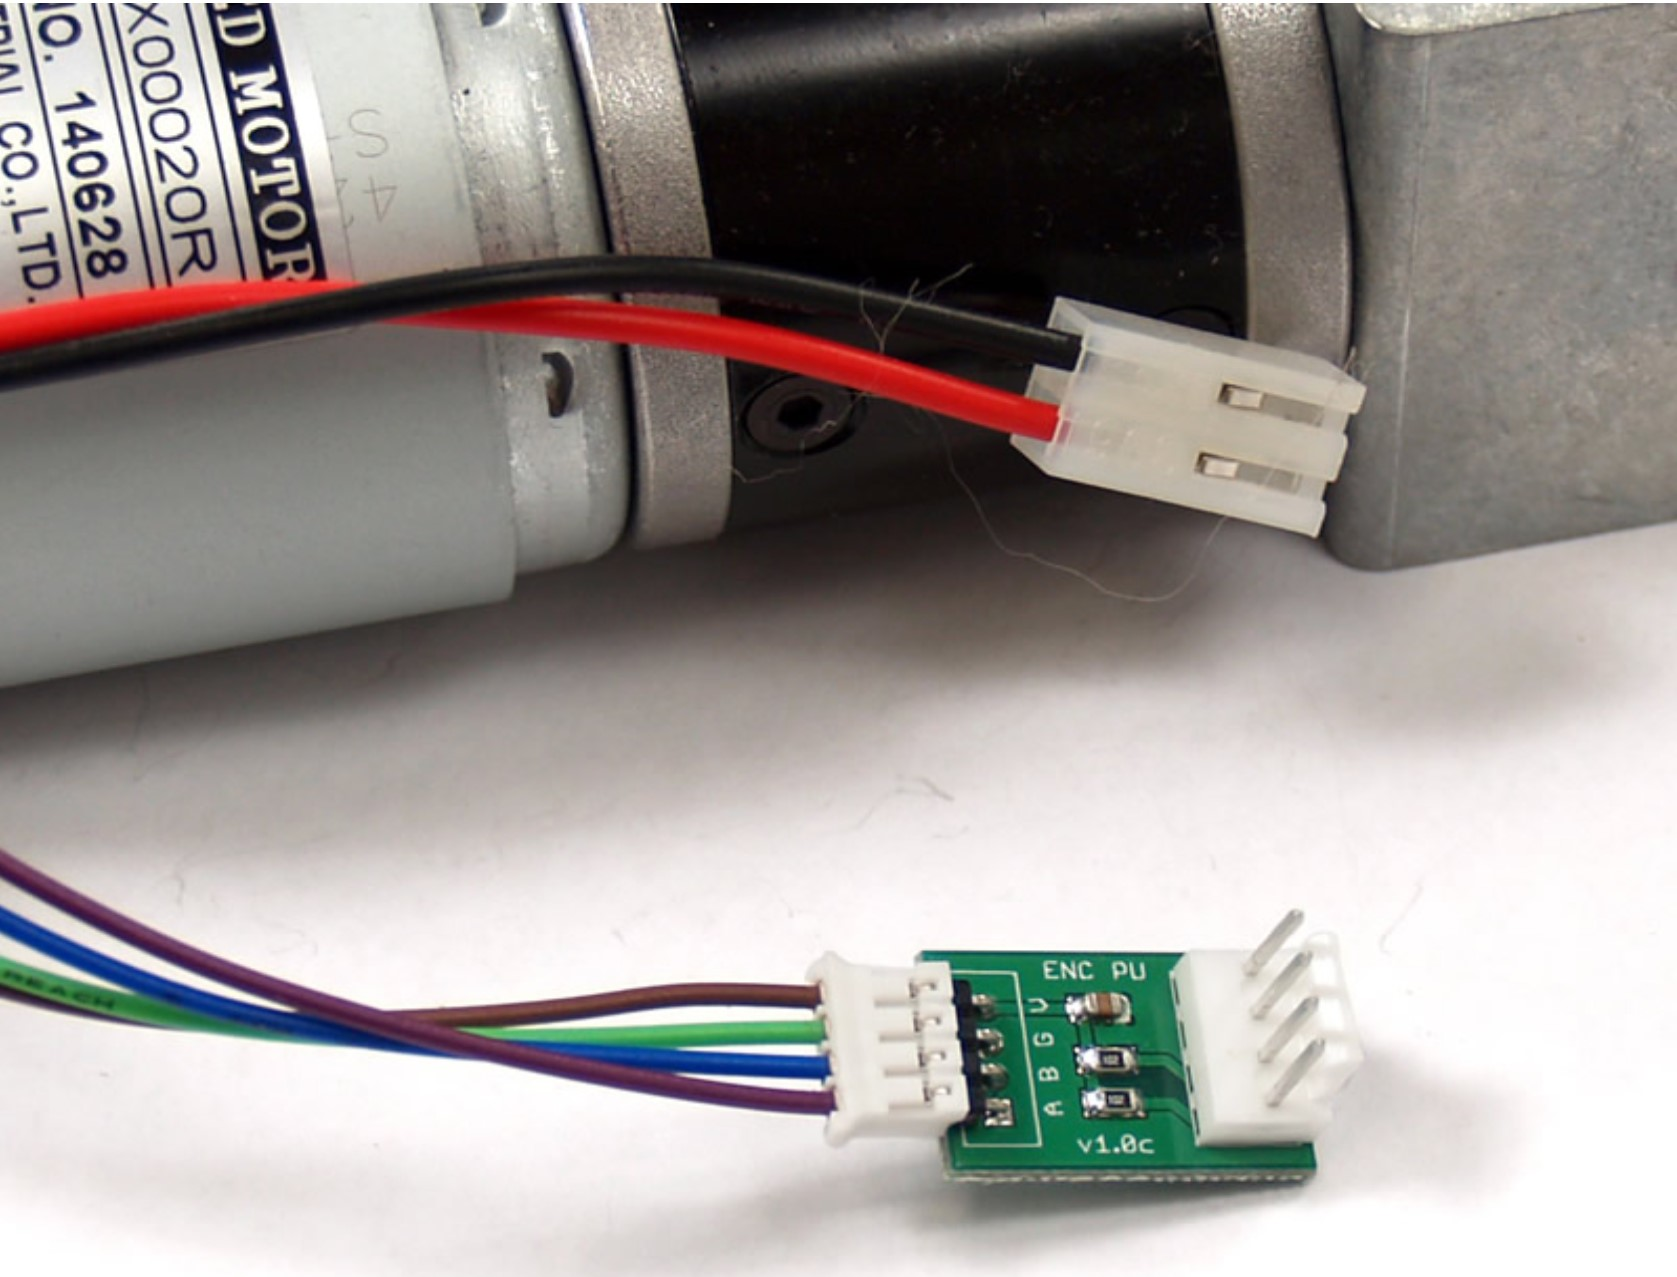
\includegraphics[width=0.45\textwidth]{figures/gearMotorPullUpBoard.jpg}} \\
\end{tabular}

\begin{tabular}{ c c }
    Cable layout & Schematic \\
    %\hline
     \raisebox{-\totalheight}{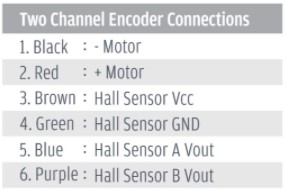
\includegraphics[width=0.45\textwidth]{figures/encoderPins.jpg}} & \raisebox{-\totalheight}{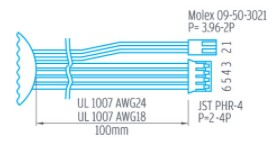
\includegraphics[width=0.45\textwidth]{figures/encoderPins2.jpg}} \\
\end{tabular}

\begin{tabular}{ c }
    Electrical caracteristics \\
    %\hline
     \raisebox{-\totalheight}{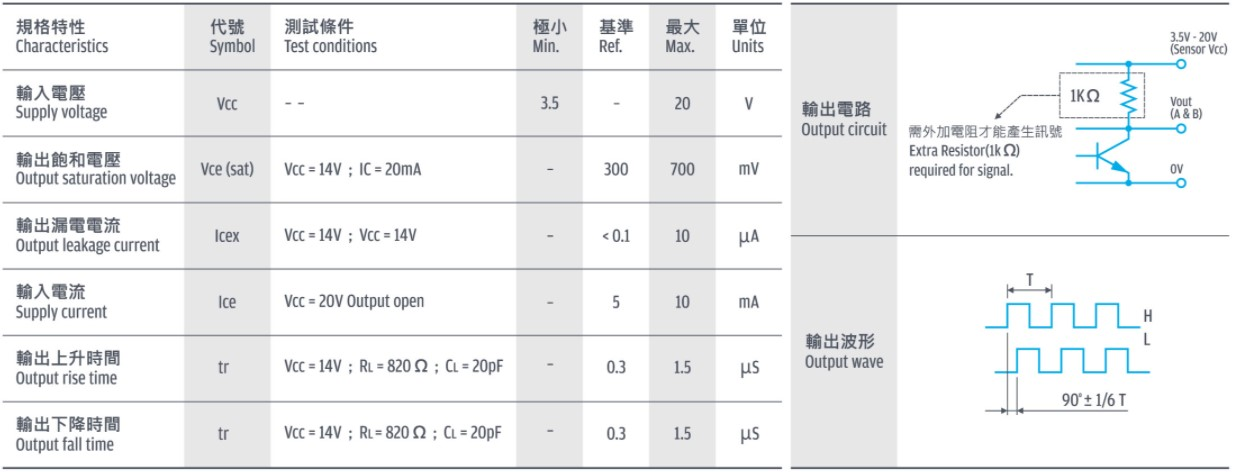
\includegraphics[width=0.9\textwidth]{figures/electricalCaracteristics.jpg}} \\
\end{tabular}

\begin{itemize}
    \item To reduce noise as much as possible in the system, twist positive and negative wires together and use ferrite beads at each motor connection.
    \item Bigger ferrite first over both wires and one smaller ferrite bead over each wire. (Don't forget the heatshrink)
\end{itemize}


%Here some examples of references \cite{Pomerleau2013,Pomerleau2014}.

% ---------------------------------------------------------------
\newpage
\section{Roboclaw 2x30A Motor Controller}%

\begin{figure}[h]
    \centering
    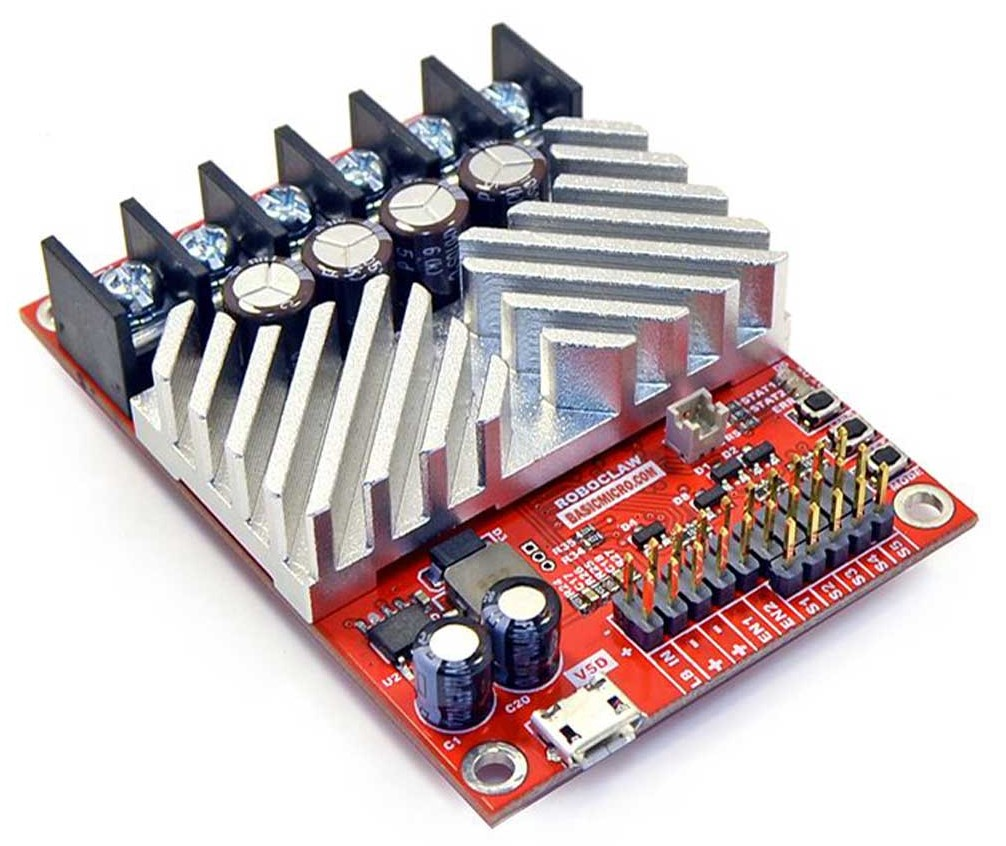
\includegraphics[width=0.3\textwidth]{figures/roboclaw.jpg}
    \caption{Motor Controller}
    \label{fig:my_label}
\end{figure}

\begin{tabular}{ c c }
    Hardware overview & Control interface \\
    %\hline
     \raisebox{-\totalheight}{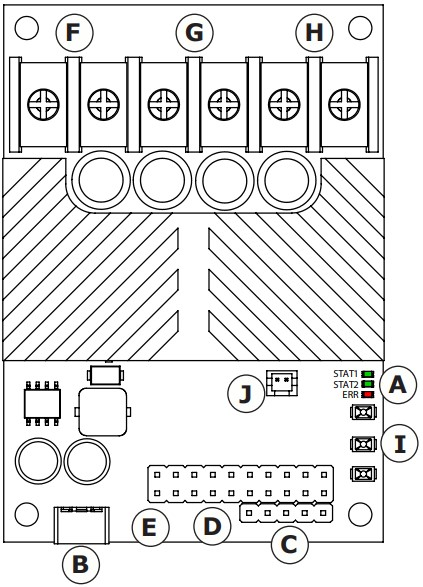
\includegraphics[width=0.30\textwidth]{figures/roboclawHardwareOverview.jpg}} & \raisebox{-\totalheight}{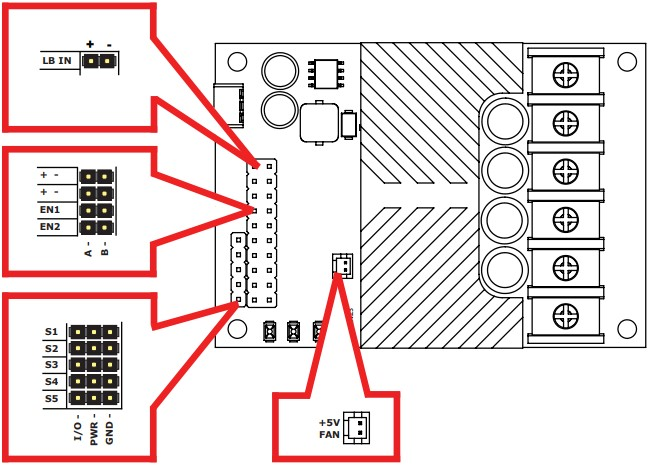
\includegraphics[width=0.55\textwidth]{figures/roboclawPinLayout.jpg}} \\
\end{tabular}

\begin{itemize}
    \item Connect batteries to the main terminal (G).
    \item Connect encoder through pull up resistor chip to pins in section D.
    \item See schematic below for details.
    \item For initial tests connect roboclaw through usb to computer (batteries have to be connected to roboclaw to function). Use motion studio to check if motors and sensors work.
\end{itemize}

\newpage
\begin{figure}[h]
    \centering
    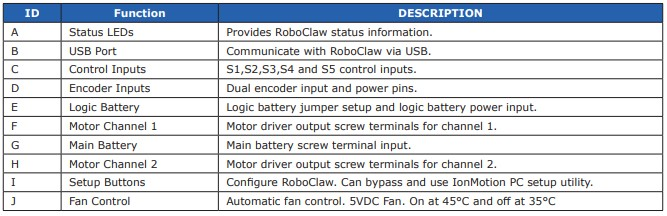
\includegraphics[width=0.9\textwidth]{figures/roboclawHardwareTable.jpg}
    \caption{Hardware overview reference table}
    \label{fig:my_label}
\end{figure}

\begin{figure}[h]
    \centering
    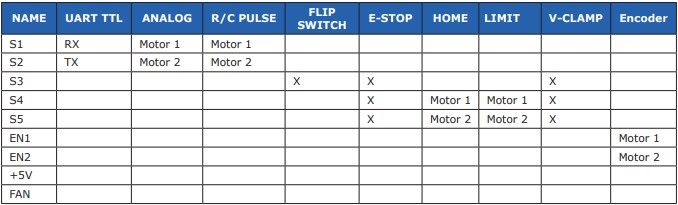
\includegraphics[width=0.9\textwidth]{figures/roboclawPinTable.jpg}
    \caption{Control interface reference table}
    \label{fig:my_label}
\end{figure}

\newpage
\begin{figure}[h]
    \centering
    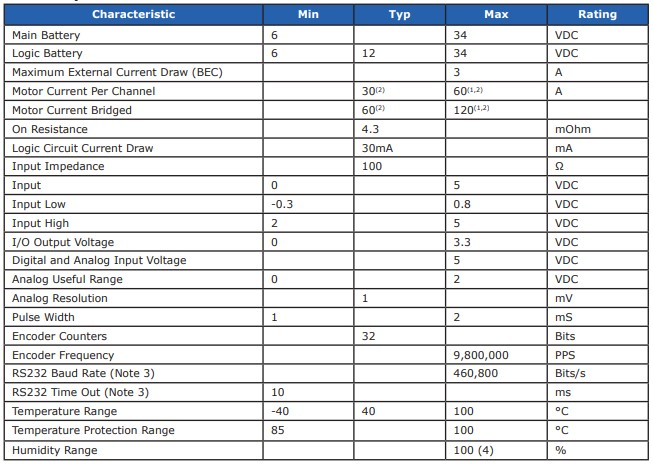
\includegraphics[width=0.9\textwidth]{figures/electricalSpecsTable.jpg}
    \caption{Electrical specifications}
    \label{fig:my_label}
\end{figure}

\newpage
\begin{figure}[h]
    \centering
    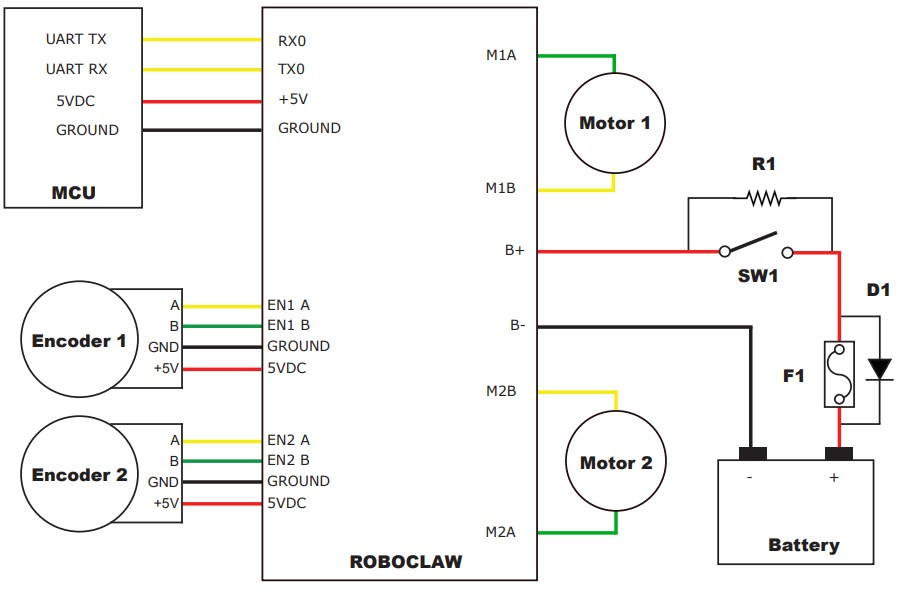
\includegraphics[width=0.9\textwidth]{figures/wiring.jpg}
    \caption{Safety wiring}
    \label{fig:my_label}
\end{figure}

% ---------------------------------------------------------------
\section{Motion studio}

% ---------------------------------------------------------------
\section{ROS Driver}

% ---------------------------------------------------------------
\section{Remote Control}

% ---------------------------------------------------------------
\printbibliography

\end{document}